\chapter{Phương pháp đề xuất}
\label{chap:method}

Chương này trình bày chi tiết phương pháp PhaBERT-CNN được đề xuất để dự đoán lối sống thực khuẩn thể từ các contig metagenomic. Phương pháp kết hợp mô hình nền tảng genome DNABERT-2 với kiến trúc chuyên biệt task-specific bao gồm mạng nơ-ron tích chập đa tỷ lệ và cơ chế attention pooling. Chương được tổ chức thành các phần chính: Phần \ref{sec:overview} giới thiệu tổng quan về phương pháp PhaBERT-CNN, bao gồm động lực thiết kế và quy trình xử lý tổng thể từ đầu vào DNA sequence đến đầu ra dự đoán lifestyle; Phần \ref{sec:data_preprocessing} mô tả quy trình thu thập và tiền xử lý dữ liệu, bao gồm nguồn dữ liệu, phương pháp tạo contig bằng sliding window, data augmentation với reverse complement, và xử lý class imbalance; Phần \ref{sec:architecture} trình bày chi tiết kiến trúc PhaBERT-CNN với ba thành phần chính (DNABERT-2 backbone, nhánh song song kép với multi-scale CNN và attention-based pooling, đầu phân loại); cuối cùng, Phần \ref{sec:training_strategy} mô tả chiến lược huấn luyện hai giai đoạn với giai đoạn khởi động và giai đoạn tinh chỉnh đầy đủ sử dụng discriminative learning rates và các kỹ thuật regularization.

\section{Tổng quan phương pháp}
\label{sec:overview}

Các phương pháp hiện có cho dự đoán lối sống thực khuẩn thể gặp phải những hạn chế quan trọng khi áp dụng trên dữ liệu di truyền được thu thập từ các mẫu trong môi trường. Các phương pháp học máy truyền thống như PHACTS\cite{mcnair2012phacts}, PhageAI\cite{tynecki2020phageai}, và BACPHLIP\cite{hockenberry2021bacphlip} yêu cầu dữ liệu di truyền đầy đủ và phụ thuộc vào việc nhận diện các protein bảo tồn, dẫn đến hiệu suất giảm mạnh trên các đoạn dữ liệu di truyền ngắn. Các phương pháp học sâu gần đây như DeePhage\cite{wu2021deephage} sử dụng phương pháp mã hóa one-hot đạt độ chính xác 78.07--89.09\% trên các contig 100--1800 bp nhưng không tận dụng được đặc trưng genomic tiền huấn luyện. PhaTYP\cite{shang2023phatyp} cải thiện hiệu suất lên 91.02\% nhưng phụ thuộc vào công cụ gán nhãn gene (Prodigal\cite{hyatt2010prodigal}), dẫn đến hiệu suất giảm đáng kể trên các contig ngắn. DeepPL\cite{zhang2024deeppl} sử dụng DNABERT với tokenization 6-mer đạt độ chính xác 94.65\%, tuy nhiên các phương pháp k-mer chồng lấn gặp phải vấn đề rò rỉ thông tin và kém hiệu quả về mặt tính toán.

Để giải quyết các hạn chế trên, chúng tôi đề xuất PhaBERT-CNN, một phương pháp học sâu kết hợp mô hình nền tảng genome DNABERT-2\cite{zhou2023dnabert} với kiến trúc mạng nơ-ron tích chập đa tỷ lệ và cơ chế attention pooling. Phương pháp được thiết kế với bốn ưu điểm chính: (1) \textbf{Độc lập với dự đoán gene}—hoạt động trực tiếp trên chuỗi DNA thô thông qua BPE tokenization, không phụ thuộc vào công cụ dự đoán gene, cho phép dự đoán chính xác ngay cả trên các contig ngắn thiếu vùng mã hóa protein hoàn chỉnh; (2) \textbf{Loại bỏ rò rỉ thông tin}—BPE tokenization tạo ra các token con không chồng lấn với độ dài biến đổi, giảm độ dài chuỗi khoảng 5 lần và loại bỏ hoàn toàn tương quan giả tạo vốn có trong các phương pháp k-mer chồng lấn; (3) \textbf{Tận dụng đặc trưng genomic tiền huấn luyện}—DNABERT-2 đã được tiền huấn luyện trên kho dữ liệu genome đa loài, cho phép mô hình nắm bắt các mẫu ngữ cảnh phức tạp và dấu hiệu tiến hóa mà không cần dữ liệu huấn luyện quy mô lớn cho tác vụ cụ thể.

Hình~\ref{fig:phabert_pipeline} minh họa quy trình xử lý tổng thể của PhaBERT-CNN,  bao gồm bốn giai đoạn chính. Đầu tiên, chuỗi DNA đầu vào được nén bởi BPE. Tiếp theo, DNABERT-2 chuyển đổi chuỗi token thành các biểu diễn ngữ cảnh 768 chiều cho mỗi vị trí. Các biểu diễn này sau đó được xử lý song song bởi hai nhánh: nhánh CNN đa kernel, được điều chỉnh từ kiến trúc TextCNN~\cite{kim2014convolutional} với các nhánh tích chập song song có kích thước kernel khác nhau (3, 5, 7) để trích xuất đa dạng các đặc trưng cục bộ; trong khi nhánh Attention Pooling~\cite{lin2017structured} tổng hợp thông tin toàn cục có trọng số. Cuối cùng, đặc trưng từ hai nhánh được ghép nối và đưa vào đầu phân loại để tạo ra dự đoán nhị phân giữa thực khuẩn thể độc lực và thực khuẩn thể ôn hòa. Chi tiết kiến trúc của PhaBERT-CNN được trình bày trong Phần \ref{sec:architecture}.

Về chiến lược huấn luyện, PhaBERT-CNN áp dụng quy trình hai giai đoạn nhằm tận dụng tối đa tri thức tiền huấn luyện của DNABERT-2 trong khi tránh hiện tượng quên tri thức tiền huấn luyện. Trong giai đoạn khởi động, toàn bộ tham số của DNABERT-2 được đóng băng và chỉ các lớp cho tác vụ phía sau được huấn luyện, giúp khởi tạo ổn định các thành phần mới trước khi tinh chỉnh toàn bộ mô hình. Giai đoạn tiếp theo mở khóa backbone và áp dụng tốc độ học phân biệt, tốc độ học thấp hơn cho DNABERT-2 và cao hơn cho các lớp tác vụ phía sau, để bảo toàn tri thức tiền huấn luyện của DNABERT-2 trong khi thích nghi với tác vụ phân loại lối sống. Chi tiết chiến lược huấn luyện được trình bày trong Phần \ref{sec:training_strategy}.

\begin{figure}[h]
    \centering
    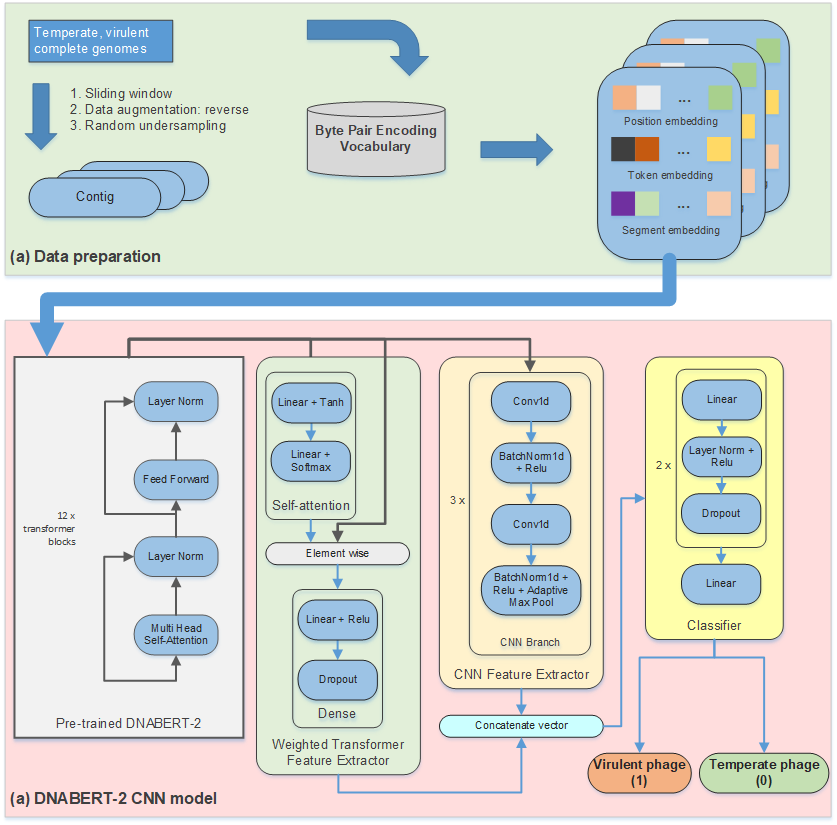
\includegraphics[width=0.9\textwidth]{imgs/my_pipeline.png}
    \caption{Quy trình xử lý tổng thể của PhaBERT-CNN cho dự đoán lối sống thực khuẩn thể}
    \label{fig:phabert_pipeline}
\end{figure}

\section{Thu thập dữ liệu và tiền xử lý}
\label{sec:data_preprocessing}

Tập dữ liệu huấn luyện được xây dựng bằng cách tích hợp và tinh chỉnh các bộ hệ gen từ hai nghiên cứu trước về phân loại lối sống thực khuẩn thể. \textbf{DeePhage}~\cite{wu2021deephage} cung cấp tập dữ liệu gồm 2 phần, phần 1 là tập được kiểm duyệt thủ công được xác minh qua đối chiếu tài liệu thực nghiệm, phần 2 là dữ liệu thu thập được từ NCBI, sử dụng phương pháp tin sinh học của Mavrich và Hatfull~\cite{mavrich2017bacteriophage} để gán nhãn. \textbf{DeepPL}~\cite{zhang2024deeppl} tiếp đó thực hiện tinh chỉnh và thu thập thêm dữ liệu từ NCBI. Sau khi tổng hợp, tập dữ liệu kết hợp bao gồm \textbf{2,241 hệ gen phage hoàn chỉnh}, trong đó 707 phage thuộc lớp temperate (nhãn 0) và 1,534 phage thuộc lớp virulent (nhãn 1). Tỷ lệ nhãn 1:0 là $\approx$ 2:1 cho thấy sự mất cân bằng nhẹ và cần được xử lý trong quá trình huấn luyện. Để đảm bảo kết quả đánh giá, học viên sử dụng \textbf{stratified 5-fold cross-validation} với tỷ lệ dữ liệu trong tập huấn luyện và kiểm thử là 8:2 trong mỗi fold, đảm bảo phân phối lớp được duy trì nhất quán qua các lần chia.

Quy trình tiền xử lý dữ liệu bao gồm ba bước liên tiếp: tạo contig bằng cửa sổ trượt, tăng cường dữ liệu với đảo ngược chuỗi, và xử lý mất cân bằng dữ liệu với phương pháp Random Sampling. \textbf{Bước 1: Tạo contig bằng phương pháp cửa sổ trượt.} Trong thực tế, dữ liệu thực khuẩn thu được từ metagenomic thường ở dạng các đoạn DNA ngắn không hoàn chỉnh. Để mô phỏng kịch bản này, học viên tạo contig từ bộ gen thực khuẩn hoàn chỉnh bằng phương pháp cửa sổ trượt: với mỗi hệ gen, độ dài cửa sổ được lấy mẫu ngẫu nhiên từ phân phối chuẩn $\mathcal{N}(\mu_{\text{group}}, \sigma_{\text{group}}^2)$ và được giới hạn trong phạm vi của nhóm tương ứng; vị trí bắt đầu của cửa sổ tiếp theo được tính bằng $\text{pos} \leftarrow \text{pos} + \text{length} \times (1 - \text{overlap\_ratio}_{\text{group}})$, tạo ra sự chồng lấn có kiểm soát giữa các contig liên tiếp. Học viên chia contig thành bốn nhóm độ dài A (100--400 bp), B (400--800 bp), C (800--1200 bp), và D (1200--1800 bp) với tham số được trình bày trong Bảng~\ref{tab:sliding_window_params}. Overlap ratio tăng dần theo độ dài nhóm: nhóm ngắn (A) dùng overlap thấp để tránh tạo quá nhiều contig tương tự và giảm dư thừa, trong khi nhóm dài (D) dùng overlap cao hơn để tăng số lượng mẫu và đa dạng hóa dữ liệu, đặc biệt quan trọng vì contig dài tự nhiên ít hơn. \textbf{Bước 2: Tăng cường dữ liệu với đảo ngược chuỗi.} DNA có cấu trúc sợi đôi, trong đó cả hai hướng đọc đều mang thông tin sinh học tương đương. Tận dụng đặc tính này, với mỗi contig chúng tôi tạo thêm chuỗi đảo ngược với quy tắc bổ sung: $A \leftrightarrow T$, $C \leftrightarrow G$. Nếu trong chuỗi có $U$ thì sẽ xử lý như là với $T$. Ví dụ:
\begin{align*}
    \text{Chuỗi gốc:}          & \quad \text{ATCGATCG} \\
    \text{Chuỗi bổ sung:}      & \quad \text{TAGCTAGC} \\
    \text{Đảo ngược bổ sung:}  & \quad \text{CGATCGAT}
\end{align*}
Phép biến đổi này tăng gấp đôi kích thước bộ dữ liệu mà không cần thu thập thêm dữ liệu, đồng thời giúp mô hình học được tính bất biến theo hướng đọc, phản ánh thực tế dữ liệu có thể đến từ cả hai sợi của DNA. \textbf{Bước 3: Xử lý mất cân bằng dữ liệu bằng Random Undersampling.} Sau khi thực hiện tăng cường dữ liệu, tập dữ liệu vẫn duy trì tỷ lệ virulent:temperate $\approx$ 2:1, có thể dẫn đến mô hình bị thiên lệch về lớp đa số trong quá trình huấn luyện. Để giải quyết vấn đề này, học viên áp dụng Random Undersampling trên tập huấn luyện: giữ nguyên toàn bộ mẫu của lớp thiểu số (temperate) và ngẫu nhiên chọn số lượng mẫu tương đương từ lớp đa số (virulent), tạo ra tập huấn luyện cân bằng với tỷ lệ 1:1. Phương pháp này được chọn vì đơn giản, hiệu quả, và phù hợp với mức độ mất cân bằng không quá nghiêm trọng (2:1). Quan trọng là Random Undersampling chỉ được áp dụng trên tập huấn luyện; tập kiểm định giữ nguyên phân phối gốc để đánh giá hiệu suất trên phân phối thực tế. Bảng~\ref{tab:dataset_statistics} tổng hợp thống kê số lượng contig sau tăng cường dữ liệu (trước Random Undersampling).

\begin{table}[h]
    \centering
    \caption{Tham số sliding window cho các nhóm độ dài contig}
    \label{tab:sliding_window_params}
    \begin{tabular}{lcccc}
        \toprule
        \textbf{Nhóm} & \textbf{Phạm vi (bp)} & \textbf{$\mu$ (bp)} & \textbf{$\sigma$ (bp)} & \textbf{Overlap ratio} \\
        \midrule
        A             & 100--400              & 250                 & 75                     & 10\%                   \\
        B             & 400--800              & 600                 & 100                    & 20\%                   \\
        C             & 800--1200             & 1000                & 100                    & 30\%                   \\
        D             & 1200--1800            & 1500                & 150                    & 40\%                   \\
        \bottomrule
    \end{tabular}
\end{table}

% TODO: cập nhật số liệu thực tế sau khi chạy thực nghiệm
\begin{table}[h]
    \centering
    \caption{Thống kê số lượng contig sau augmentation (trước undersampling)}
    \label{tab:dataset_statistics}
    \begin{tabular}{lrrrr}
        \toprule
        \textbf{Nhóm}    & \textbf{Temperate} & \textbf{Virulent} & \textbf{Total} & \textbf{Ratio (V:T)} \\
        \midrule
        A (100--400 bp)  & \textbf{TODO}      & \textbf{TODO}     & \textbf{TODO}  & \textbf{TODO}        \\
        B (400--800 bp)  & \textbf{TODO}      & \textbf{TODO}     & \textbf{TODO}  & \textbf{TODO}        \\
        C (800--1200 bp) & \textbf{TODO}      & \textbf{TODO}     & \textbf{TODO}  & \textbf{TODO}        \\
        D (1200--1800 bp)& \textbf{TODO}      & \textbf{TODO}     & \textbf{TODO}  & \textbf{TODO}        \\
        \bottomrule
    \end{tabular}
\end{table}

\section{Kiến trúc PhaBERT-CNN}
\label{sec:architecture}

Kiến trúc PhaBERT-CNN được xây dựng từ ba thành phần chính hoạt động tuần tự: (1) DNABERT-2 backbone đóng vai trò trích xuất đặc trưng ngữ cảnh từ chuỗi DNA, (2) Mô đun Modified TextCNN tiếp tục xử lý các biểu diễn đầu ra của DNABERT-2 và (3) bộ phân loại đưa ra dự đoán nhị phân. Hình~\ref{fig:architecture_detail} minh họa kiến trúc tổng thể của mô hình.

\begin{figure}[h]
    \centering
    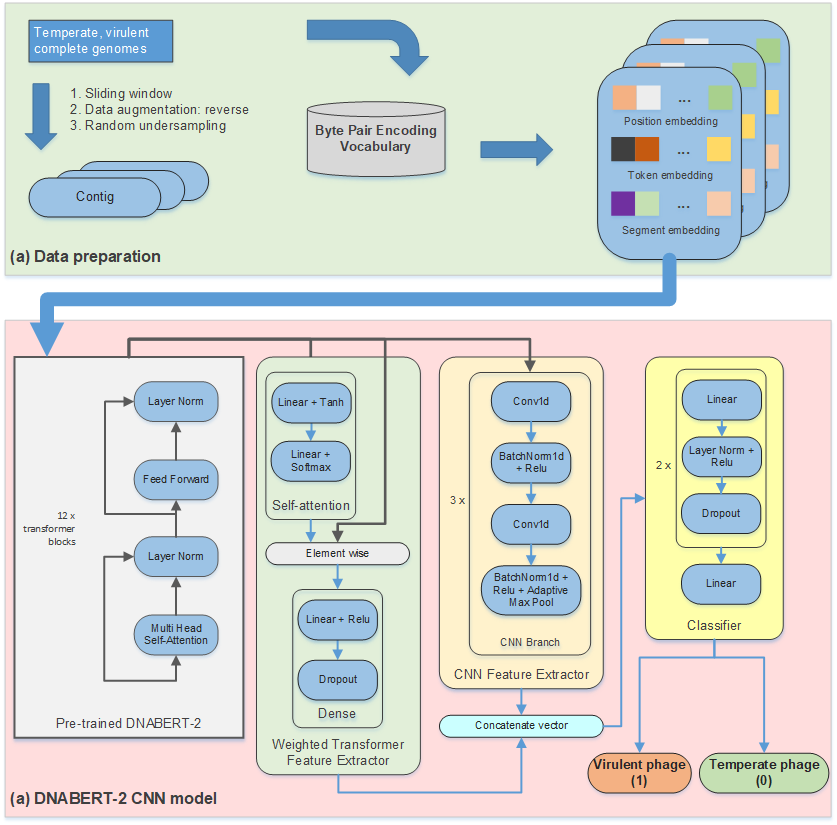
\includegraphics[width=1.0\textwidth]{imgs/my_pipeline.png}
    \caption{Kiến trúc chi tiết của PhaBERT-CNN}
    \label{fig:architecture_detail}
\end{figure}

\subsection{DNABERT-2 Backbone}

DNABERT-2~\cite{zhou2023dnabert} đóng vai trò là backbone trích xuất đặc trưng, chuyển đổi chuỗi DNA thô thành các véc-tơ 768 chiều. Chuỗi DNA đầu vào $S = \{s_1, s_2, \ldots, s_L\}$ với độ dài $L$ cặp ba-zơ trước tiên được tokenize bằng Byte Pair Encoding (BPE)\cite{sennrich2015neural}:

\begin{equation}
    T = \text{BPE}(S) = \{t_1, t_2, \ldots, t_n\}, \quad n \approx L/5
    \label{eq:bpe_tokenization}
\end{equation}

BPE tạo ra các token con không chồng lấn với độ dài biến đổi, giúp giảm độ dài chuỗi token khoảng 5 lần so với phương pháp k-mer truyền thống \cite{zhou2023dnabert}. Cách tiếp cận này không chỉ cải thiện đáng kể hiệu quả tính toán mà còn loại bỏ hiện tượng rò rỉ thông tin vốn có trong các phương pháp k-mer chồng lấn, nơi các token liền kề chia sẻ $k{-}1$ nucleotide và vô tình tiết lộ thông tin về các vị trí bị che. Chuỗi token $T$ thu được sau đó được đưa qua DNABERT-2 để tạo ra các biểu diễn ngữ cảnh:

\begin{equation}
    \mathbf{H} = \text{DNABERT-2}(T) = \{\mathbf{h}_1, \mathbf{h}_2, \ldots, \mathbf{h}_n\}, \quad \mathbf{h}_i \in \mathbb{R}^{768}
    \label{eq:dnabert2_encoding}
\end{equation}

trong đó mỗi vector $\mathbf{h}_i$ mã hóa thông tin của token tương ứng cùng mối quan hệ ngữ cảnh với các token xung quanh thông qua cơ chế tự chú ý. DNABERT-2 sử dụng Attention with Linear Biases (ALiBi)~\cite{press2021train} thay vì positional embeddings học được, cho phép mô hình xử lý các chuỗi có độ dài tùy ý mà không cần huấn luyện lại, đặc biệt quan trọng cho dữ liệu metagenomic với độ biến thiên độ dài lớn. Trong giai đoạn khởi động, toàn bộ tham số của DNABERT-2 được đóng băng; trong giai đoạn tinh chỉnh, backbone được mở khóa và cập nhật với tốc độ học thấp để bảo toàn tri thức tiền huấn luyện.

\subsection{Modified TextCNN}

Từ các biểu diễn $\mathbf{H}$ của DNABERT-2, hai nhánh song song được áp dụng để trích xuất các đặc trưng bổ sung cho nhau: nhánh CNN đa tỷ lệ nắm bắt các mẫu cục bộ ở nhiều tỷ lệ không gian, và nhánh attention pooling tổng hợp thông tin ngữ cảnh toàn cục.

\subsubsection{Nhánh CNN Đa kernel}

Nhánh CNN đa kernel được điều chỉnh từ kiến trúc TextCNN~\cite{kim2014convolutional}, vốn được đề xuất cho bài toán phân loại văn bản với các bộ lọc tích chập song song có kích thước khác nhau. So với bản gốc vốn áp dụng trực tiếp lên embedding từ tĩnh, chúng tôi thực hiện hai điều chỉnh: (1) thay thế đầu vào bằng các biểu diễn ngữ cảnh 768 chiều từ DNABERT-2, tận dụng tri thức tiền huấn luyện thay vì embedding ngẫu nhiên; (2) bổ sung thêm một lớp tích chập xếp chồng cho mỗi pathway, tạo thành hai lớp Conv1d liên tiếp nhằm tăng khả năng trích xuất đặc trưng phân cấp từ các biểu diễn genomic phức tạp~\cite{johnson2017deep}. Thiết kế đa tỷ lệ lấy cảm hứng từ kiến trúc Inception~\cite{szegedy2015going}, cho phép mô hình đồng thời nắm bắt các mẫu ở nhiều tỷ lệ không gian khác nhau trong một lần forward pass.

Cụ thể, nhánh sử dụng ba pathway tích chập song song với kích thước cửa sổ $k \in \{3, 5, 7\}$. Mỗi pathway xử lý ma trận embedding $\mathbf{H}^T \in \mathbb{R}^{768 \times n}$ (chuyển vị để phù hợp định dạng Conv1d) qua hai lớp tích chập xếp chồng với same-padding để bảo toàn chiều dài chuỗi:

\begin{align}
    \mathbf{X}^{(k)}_1 &= \text{ReLU}(\text{BatchNorm}(\text{Conv1d}_{k,768 \to 256}(\mathbf{H}^T))) \in \mathbb{R}^{256 \times n} \label{eq:cnn_layer1} \\
    \mathbf{X}^{(k)}_2 &= \text{ReLU}(\text{BatchNorm}(\text{Conv1d}_{k,256 \to 128}(\mathbf{X}^{(k)}_1))) \in \mathbb{R}^{128 \times n} \label{eq:cnn_layer2} \\
    \mathbf{f}^{(k)} &= \text{AdaptiveMaxPool1d}(\mathbf{X}^{(k)}_2) \in \mathbb{R}^{128} \label{eq:cnn_pool}
\end{align}

Lớp tích chập đầu tiên giảm chiều từ 768 xuống 256 kênh, lớp thứ hai nén tiếp xuống 128 kênh. BatchNorm1d và ReLU sau mỗi lớp ổn định quá trình huấn luyện và tăng tính phi tuyến. AdaptiveMaxPool1d trích xuất đặc trưng nổi bật nhất từ chiều chuỗi, tạo ra vector đặc trưng cố định 128 chiều bất kể độ dài contig đầu vào. Ba kernel size được chọn để nắm bắt các tín hiệu genomic ở các tỷ lệ khác nhau: \textbf{kernel size 3} phát hiện các motif cục bộ ngắn tương ứng vùng liên kết transcription factor và promoter; \textbf{kernel size 5} nắm bắt các mẫu trung gian như ribosome binding sites và các phần tử điều hòa nhỏ; \textbf{kernel size 7} nhận diện các vùng chức năng rộng hơn như integration sites và các vùng điều hòa lớn. Ba vector đặc trưng từ các pathway được ghép nối tạo thành biểu diễn CNN tổng hợp:

\begin{equation}
    \mathbf{f}_{\text{CNN}} = [\mathbf{f}^{(3)}; \mathbf{f}^{(5)}; \mathbf{f}^{(7)}] \in \mathbb{R}^{384}
    \label{eq:cnn_concat}
\end{equation}

\subsubsection{Nhánh Attention Pooling Toàn Cục}

Nhánh thứ hai lấy cảm hứng từ cơ chế tự chú ý~\cite{lin2017structured} để tổng hợp thông tin mức chuỗi từ các biểu diễn transformer, tự động gán trọng số cho tầm quan trọng của các vị trí khác nhau trên chuỗi. Cho hidden states $\mathbf{H} = \{\mathbf{h}_1, \ldots, \mathbf{h}_n\}$ từ DNABERT-2, điểm attention cho mỗi vị trí được tính qua hai lớp tuyến tính:

\begin{align}
    \mathbf{e}_t &= \tanh(\mathbf{W}_a \mathbf{h}_t + \mathbf{b}_a), \quad \mathbf{e}_t \in \mathbb{R}^{64} \label{eq:attn_hidden} \\
    s_t &= \mathbf{w}_s^T \mathbf{e}_t + b_s, \quad s_t \in \mathbb{R} \label{eq:attn_score} \\
    \alpha_t &= \frac{\exp(s_t)}{\sum_{t'=1}^{n} \exp(s_{t'})}, \quad \alpha_t \in [0, 1], \; \sum_t \alpha_t = 1 \label{eq:attn_weights}
\end{align}

trong đó $\mathbf{W}_a \in \mathbb{R}^{64 \times 768}$, $\mathbf{b}_a \in \mathbb{R}^{64}$ là tham số lớp chiếu ẩn, và $\mathbf{w}_s \in \mathbb{R}^{64}$, $b_s \in \mathbb{R}$ là tham số lớp tính điểm scalar. Biểu diễn chuỗi ngữ cảnh được tạo bằng tổng có trọng số:

\begin{equation}
    \mathbf{v} = \sum_{t=1}^{n} \alpha_t \mathbf{h}_t \in \mathbb{R}^{768}
    \label{eq:attn_aggregate}
\end{equation}

Biểu diễn tổng hợp $\mathbf{v}$ sau đó được chiếu tuyến tính xuống không gian đặc trưng compact:

\begin{equation}
    \mathbf{f}_{\text{attn}} = \text{Dropout}(\text{ReLU}(\mathbf{W}_p \mathbf{v} + \mathbf{b}_p)) \in \mathbb{R}^{128}
    \label{eq:attn_proj}
\end{equation}

trong đó $\mathbf{W}_p \in \mathbb{R}^{128 \times 768}$, $\mathbf{b}_p \in \mathbb{R}^{128}$, và dropout rate = 0.1. So với max/average pooling thông thường, attention pooling có ba ưu điểm chính: \textbf{trọng số động}—cơ chế attention học cách gán trọng số cho tầm quan trọng của các vị trí dựa trên ngữ cảnh thay vì xử lý đồng đều; \textbf{khả năng diễn giải}—các trọng số $\{\alpha_t\}$ có thể được trực quan hóa để hiểu mô hình tập trung vào vùng genomic nào; \textbf{bất biến với độ dài}—attention tự nhiên xử lý các chuỗi có độ dài biến đổi mà không cần padding hay truncation.

\subsection{Kết Hợp Đặc Trưng và Đầu Phân Loại}

Đầu ra từ cả hai nhánh được ghép nối để tạo biểu diễn tổng hợp:

\begin{equation}
    \mathbf{f}_{\text{combined}} = [\mathbf{f}_{\text{attn}}; \mathbf{f}_{\text{CNN}}] = [\mathbf{f}_{\text{attn}}; \mathbf{f}^{(3)}; \mathbf{f}^{(5)}; \mathbf{f}^{(7)}] \in \mathbb{R}^{512}
    \label{eq:feature_fusion}
\end{equation}

Vector 512 chiều này kết hợp cả ngữ cảnh toàn cục từ nhánh attention (128 chiều) và đặc trưng cục bộ đa tỷ lệ từ các nhánh CNN (384 chiều). Biểu diễn tổng hợp được đưa qua đầu phân loại gồm ba lớp tuyến tính với kích thước giảm dần $512 \to 256 \to 64 \to 2$:

\begin{align}
    \mathbf{z}_1 &= \text{Dropout}(\text{ReLU}(\text{LayerNorm}(\mathbf{W}_1 \mathbf{f}_{\text{combined}} + \mathbf{b}_1))), \quad \mathbf{z}_1 \in \mathbb{R}^{256} \label{eq:cls_layer1} \\
    \mathbf{z}_2 &= \text{Dropout}(\text{ReLU}(\mathbf{W}_2 \mathbf{z}_1 + \mathbf{b}_2)), \quad \mathbf{z}_2 \in \mathbb{R}^{64} \label{eq:cls_layer2} \\
    \mathbf{z}_3 &= \mathbf{W}_3 \mathbf{z}_2 + \mathbf{b}_3 \in \mathbb{R}^{2} \label{eq:cls_output}
\end{align}

trong đó $\mathbf{W}_1 \in \mathbb{R}^{256 \times 512}$, $\mathbf{W}_2 \in \mathbb{R}^{64 \times 256}$, $\mathbf{W}_3 \in \mathbb{R}^{2 \times 64}$ là các ma trận trọng số, và dropout rate = 0.1 được áp dụng sau mỗi lớp ẩn để regularization. Layer Normalization sau lớp đầu tiên ổn định quá trình huấn luyện. Logit nhị phân $\mathbf{z}_3 = [z_{\text{temp}}, z_{\text{vir}}]$ được chuyển thành xác suất qua softmax:

\begin{equation}
    P(\text{virulent} | S) = \frac{\exp(z_{\text{vir}})}{\exp(z_{\text{temp}}) + \exp(z_{\text{vir}})}
    \label{eq:softmax}
\end{equation}

Dự đoán cuối cùng là $\hat{y} = \argmax(\operatorname{softmax}(\mathbf{z}_3))$, trong đó $\hat{y} = 0$ tương ứng với thực khuẩn thể ôn hòa (temperate) và $\hat{y} = 1$ tương ứng với thực khuẩn thể độc lực (virulent).

\section{Chiến lược huấn luyện và tinh chỉnh}
\label{sec:training_strategy}

Việc fine-tune một mô hình tiền huấn luyện với các lớp task-specific được khởi tạo ngẫu nhiên có thể gây ra bất ổn định trong quá trình huấn luyện do sự không tương thích gradient giữa các trọng số tiền huấn luyện và các trọng số ngẫu nhiên. Để giải quyết vấn đề này, học viên áp dụng chiến lược huấn luyện hai giai đoạn (two-phase progressive fine-tuning): giai đoạn warm-up khởi tạo các lớp task-specific trước, sau đó giai đoạn fine-tuning đầy đủ với discriminative learning rates tối ưu hóa toàn bộ kiến trúc.

\subsection{Giai Đoạn 1: Warm-up}

Trong giai đoạn warm-up, toàn bộ tham số của DNABERT-2 backbone (117M tham số) được đóng băng, chỉ các lớp task-specific (multi-scale CNN, attention pooling, và đầu phân loại, tổng cộng khoảng 2.08M tham số) được huấn luyện trong 1 epoch. Mục đích của giai đoạn này là cho phép các lớp được khởi tạo ngẫu nhiên học được cấu hình tham số phù hợp với các biểu diễn DNABERT-2 đã đóng băng trước khi thực hiện bất kỳ cập nhật nào lên các trọng số tiền huấn luyện. Việc đóng băng backbone ngăn chặn các gradient lớn từ các lớp ngẫu nhiên lan truyền ngược qua DNABERT-2, bảo toàn tri thức genomic đã học. Các lớp task-specific được tối ưu hóa bằng AdamW~\cite{loshchilov2017decoupled} với learning rate $2 \times 10^{-3}$, weight decay $1 \times 10^{-4}$, và các hệ số momentum $\beta_1 = 0.9$, $\beta_2 = 0.999$. Lịch trình learning rate theo one-cycle~\cite{smith2019super} với 30\% warm-up period, initial division factor 5, và final division factor 10 đảm bảo hội tụ ổn định trong giai đoạn ngắn này.

\subsection{Giai Đoạn 2: Fine-tuning Đầy Đủ}

Sau giai đoạn warm-up, toàn bộ kiến trúc được mở khóa và tối ưu hóa với discriminative learning rates—chiến lược áp dụng learning rate khác nhau cho các thành phần khác nhau của mô hình~\cite{howard2018universal}. Cụ thể, các tham số DNABERT-2 được cập nhật với learning rate thấp $1 \times 10^{-5}$ (weight decay $1 \times 10^{-5}$) để cho phép thích nghi nhẹ nhàng với tác vụ phân loại phage mà không làm mất các mẫu genomic tổng quát đã học trong quá trình tiền huấn luyện. Trong khi đó, các lớp task-specific (CNN, attention, đầu phân loại) nhận learning rate cao hơn 10 lần là $1 \times 10^{-4}$ (weight decay $1 \times 10^{-4}$) để cho phép tối ưu hóa tích cực hơn nhằm nắm bắt các đặc trưng đặc thù của lối sống phage. Cả hai nhóm tham số đều sử dụng AdamW với $\beta_1 = 0.9$, $\beta_2 = 0.999$, $\epsilon = 10^{-6}$. Giai đoạn fine-tuning kéo dài tối đa 10 epoch với lịch trình one-cycle (10\% warm-up period, initial division factor 5, final division factor 50) và early stopping dựa trên validation accuracy với patience 3 epoch để ngăn overfitting và chọn checkpoint tốt nhất.

\subsection{Hàm Mất Mát và Kỹ Thuật Regularization}

Học viên sử dụng binary cross-entropy loss làm mục tiêu tối ưu hóa cho tác vụ phân loại nhị phân:

\begin{equation}
    \mathcal{L}_{\text{BCE}} = -\frac{1}{N} \sum_{i=1}^{N} \left[ y_i \log(\hat{y}_i) + (1 - y_i) \log(1 - \hat{y}_i) \right]
    \label{eq:bce_loss}
\end{equation}

trong đó $N$ là batch size, $y_i \in \{0, 1\}$ là nhãn thực (0 = temperate, 1 = virulent), và $\hat{y}_i = P(\text{virulent} | S_i)$ là xác suất dự đoán. Để ngăn overfitting, học viên kết hợp nhiều kỹ thuật regularization: \textbf{Weight Decay} thông qua AdamW với $\lambda = 1 \times 10^{-4}$ cho các lớp task-specific và $\lambda = 1 \times 10^{-5}$ cho DNABERT-2; \textbf{Dropout} với rate = 0.1 được áp dụng sau attention pooling và trong đầu phân loại; \textbf{Layer Normalization} ổn định quá trình huấn luyện và cải thiện khả năng tổng quát hóa; và \textbf{Early Stopping} dừng huấn luyện khi validation performance không cải thiện sau 3 epoch liên tiếp. Ngoài ra, học viên sử dụng Automatic Mixed Precision (AMP) để giảm tiêu thụ bộ nhớ và tăng tốc tính toán, kết hợp với gradient accumulation (4 bước, batch size vật lý 8 mẫu/GPU) để mô phỏng effective batch size 32 trên bộ nhớ GPU hạn chế.

Về hạ tầng tính toán, các thực nghiệm được thực hiện trên GPU NVIDIA RTX 5070Ti với CPU Intel i5 13500 và 64GB RAM.

\section{Kết luận chương}

Chương này đã trình bày phương pháp PhaBERT-CNN qua bốn phần chính. Phần~\ref{sec:data_preprocessing} mô tả quy trình xây dựng tập dữ liệu từ 2,241 hệ gen phage hoàn chỉnh thông qua sliding window contig generation, tăng cường dữ liệu bằng reverse complement, và cân bằng lớp bằng Random Undersampling. Phần~\ref{sec:architecture} trình bày kiến trúc PhaBERT-CNN với DNABERT-2 làm backbone trích xuất biểu diễn ngữ cảnh, tiếp theo là mô đun Modified TextCNN gồm nhánh CNN đa tỷ lệ ($k \in \{3, 5, 7\}$) và nhánh attention pooling xử lý song song, tạo ra biểu diễn tổng hợp 512 chiều đưa qua đầu phân loại. Phần~\ref{sec:training_strategy} mô tả chiến lược huấn luyện hai giai đoạn: warm-up với backbone đóng băng để ổn định các lớp task-specific, sau đó fine-tuning đầy đủ với discriminative learning rates để bảo toàn tri thức tiền huấn luyện trong khi thích nghi với tác vụ phân loại lối sống. Chương tiếp theo trình bày kết quả thực nghiệm đánh giá hiệu suất của PhaBERT-CNN so với các phương pháp tiên tiến trên bốn nhóm độ dài contig.